\chapter{Privacyrisico's bij klassieke aanbevelingsystemen}
\label{privacyklassiek}

\section{Klassieke aanbevelingssystemen}
\label{sec:klassiek}
De verschillende soorten aanbevelingssystemen worden besproken, elke soort krijgt een korte uitleg waarin de werking ervan aan bod komt. Voor meer informatie omtrent de precieze werking wordt doorverwezen naar de vakliteratuur. \\Er wordt een onderscheid gemaakt tussen de volgende types.
\subsection{Niet-gepersonaliseerde statistieken}
Dit is de meest eenvoudige vorm van een aanbevelingssysteem. Bij deze statistieken wordt dus geen rekening gehouden met de beoordelingen of persoonlijke smaak van de gebruiker voor wie de aanbevelingen bedoeld zijn. Dit zijn statistieken zoals het gemiddelde aantal sterren beoordeeld door de hele community of items met het grootste aantal "vind-ik-leuk"'s. Andere statistieken die populair zijn, zijn productassociaties in de vorm van “mensen die x leuk vonden, vonden ook y leuk”. Externe community-data, zoals bijvoorbeeld meest verkochte items, wordt ook gebruikt.  Hoewel de niet-gepersonaliseerde statistieken duidelijk hun beperkingen hebben, zijn ze effici\"ent en kunnen ze erg nuttig zijn. 
\subsection{Content-based recommenders}
Het basisidee van inhoud-gebaseerde aanbevelingssystemen is om items te modelleren als vector in een meerdimensionale ruimte. Deze ruimte heeft als dimensies de relevante attributen van de items. De smaak van de gebruiker wordt ook voorgesteld als vector in deze ruimte, de \textit{uservector}. De uservector wordt opgesteld door zijn ratings van items die bepaalde attributen hebben. De interessante items worden meestal gevonden door die items te nemen waarvan de hoek tussen de itemvector en de uservector klein is. 
\subsection{Kennis-gebaseerde recommenders}
De gebruiker die aanbevelingen vraagt zal zijn voorkeuren aan het systeem geven. De gebruiker kan op de aangeboden items feedback geven zodat het systeem zijn aanbevelingen kan aanpassen.
\subsection{Collaborative Filtering recommenders}
\subsubsection{User-User Collaborative recommenders}
Bij user-user collaborative recommenders wordt de smaak van gebruikers vergeleken op basis van hun gegeven ratings met een  correlatieco\"effici\"ent zoals deze van Pearson. Als een gebruiker aanbevelingen vraagt, worden de gebruikers met een gelijkaardige smaak bepaald. De score voor een item wordt berekend door het gewogen gemiddelde te nemen van de scores voor dat item van de gebruikers met gelijkaardige smaak.
\subsubsection{Item-Item Collaborative recommenders}
Om een score voor een item te vinden voor een gebruiker wordt eerst gekeken naar de items waar hij wel een rating voor heeft. Indien het gezochte item volgens andere gebruikers gelijkaardig is (een gelijkaardige score heeft voor hen) aan wel beoordeelde items, neemt men het gewogen gemiddelde van de ratings van deze items.
\subsection{Andere aanbevelingssystemen}
\subsubsection{Demografic recommenders}
Als een persoonlijke voorkeur niet gekend is wordt afgegaan op kenmerken als leeftijd, geslacht en land van herkomst om aanbevelingen te genereren op basis van een stereotype.
\subsubsection{Social recommenders}
Deze aanbevelingssystemen maken gebruik van de vriendschapsbanden van een sociaal netwerk omdat aangenomen wordt dat vrienden gelijkaardige interesses hebben.
\subsubsection{Hybrid recommenders}
Zoals de naam aangeeft worden hier verschillende aanbevelingssystemen samen gecombineerd. Dit heeft als doel betere aanbevelingen te maken en de nadelen van de onderliggende systemen weg te werken.

\subsection{Singular Value Decomposition}
Singular Value Decomposition of singulierewaardenontbinding is een wiskundige techniek die toelaat aanbevelingen bij  collaborative filtering sneller te berekenen. De wiskundige basis ligt in de mogelijkheid een $m \times n$ matrix A op te splitsen in een product van drie matrices, respectievelijk een $m \times r$ matrix U, een $r \times r$ matrix $\sum$ met de singuliere waarden op de diagonaal en een $n \times r$ matrix V. 

\begin{figure}[htpb]   
    \label{Figuur::svd}      
  \begin{center}    
 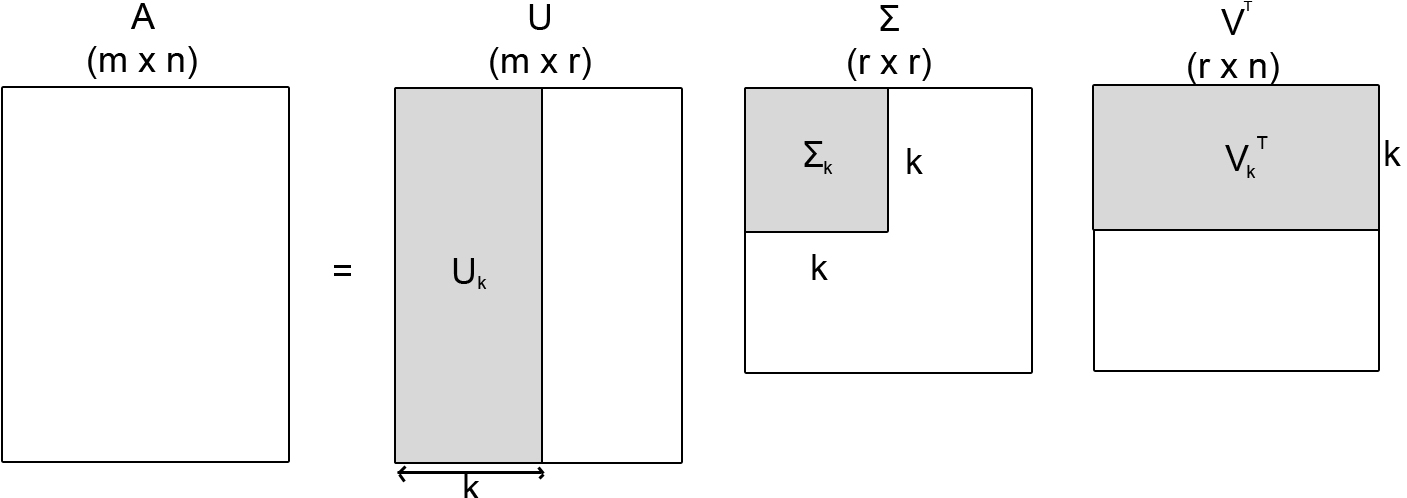
\includegraphics[scale=0.3]{fig/svd}    
  \end{center}   
    
   \end{figure}

 De singuliere waarden op de diagonaal van $\sum$ geven de belangrijkheid van deze bepaalde dimensie aan. Een deel van deze waarden is dicht bij 0 en dus kunnen deze  dimensies verwaarloosd worden en de matrix verkleind worden naar k rijen en kolommen. De scores in de U en de V matrix op deze verwaarloosde dimensies kunnen ook weggelaten worden. 
Deze techniek kan uitgevoerd worden op een traditionele userratingmatrix. Zonder SVD worden smaken van gebruikers vastgelegd als scores op bepaalde trefwoorden, zoals bij films bijvoorbeeld 5 \% comedie. Met SVD wordt de smaak van een gebruiker uitgedrukt in een kleiner aantal dimensies die een combinatie zijn van verschillende trefwoorden zonder verlies van veel informatie. Dit zorgt ervoor dat de data compacter kan worden bijgehouden en het algoritme minder computationeel werk heeft. Hierbij worden U de user-feature matrix en V de item-feature matrix genoemd.


\section{Evaluatie aanbevelingssystemen}
Een veelgebruikte basismetriek is Mean Absolute Error (MAE) of de gemiddelde absolute fout. Een rating voor een item wordt onzichtbaar gemaakt voor het systeem, waarna het systeem aangeeft welke score het zou geven op basis van alle andere bekende ratings. Het verschil tussen de vermomde score en de geraadde score is dus de fout. We berekenen het gemiddelde van de fouten voor elke rating en zo bekomen we het MAE. Een vergelijkbaar alternatief is de Mean Squared Error (MSE), die door kwadratering de grote fouten meer afstraft. De Root Mean Squared Error (RMSE) is hiervan de vierkantswortel zodat er een waarde bekomen wordt in de meer intu\"itieve originele schaal.
\begin{equation}
MAE = \frac{\sum_{ratings} (prediction - rating)}{\#ratings}
\end{equation}
\begin{equation}MSE = \frac{\sum_{ratings} (prediction - rating)^2}{\#ratings}
\end{equation}
\begin{equation}
RMSE = \sqrt{MSE}
\end{equation}
\textit{Precision} en \emph{recall} zijn ook veelgebruikte metrieken bij \emph{Information Retrieval} technieken. Ze focussen in tegenstelling tot de vorige metrieken niet op de nauwkeurigheid van een voorspellingswaarde. Precision en recall tonen respectievelijk hoeveel van de aanbevolen termen relevant zijn en het percentage van relevante items dat effectief wordt aanbevolen.


\section{Privacy}
\label{sec:privacy}
Zoals eerder gezegd bestaat er een wisselwerking tussen privacy en accuraatheid van de aanbevelingen. Hier gaan we even in op wat men precies bedoelt met privacy. Privacy op het internet betekent privacy van informatie. In de literatuur verwijst men vaak naar de definitie van het Information Infrastructure Task Force (IITF).

 \begin{quotation}
"Privacy van informatie is het recht van een individu om controle uit te oefenen op de voorwaarden waaronder zijn persoonlijke informatie verzameld, gebruikt of bekendgemaakt wordt." \\-- Information Infrastructure Task Force \cite{pirs}
 \end{quotation}
Informatie wordt door een individu altijd gedeeld binnen een bepaalde \textit{scope}. Een scope wordt afgebakend door de grootte van het publiek, de manier waarop de informatie gebruikt mag worden en hoe lang dit mag.  Privacy betekent in deze context dus de informatie in dezelfde scope te houden als vooropgesteld door de persoon die informatie verstrekte \cite{pirs}.\\
Privacy van aanbevelingssystemen kan worden opgedeeld in twee soorten. Er is \textit{user-user privacy}, met betrekking tot de privacy tussen gebruikers onderling. Bij user-user privacy gaat het om wat een gebruiker online allemaal kan te weten komen over het gedrag van andere gebruikers. Sommige websites tonen de ratings en persoonlijke voorkeuren publiek maar bij andere sites is de vooropgestelde scope veel kleiner en deze houden persoonlijke voorkeuren priv\'e of onder vrienden.  

\begin{figure}[htpb]   
    \label{Figuur::usersystemprivacy}      
  \begin{center}    
 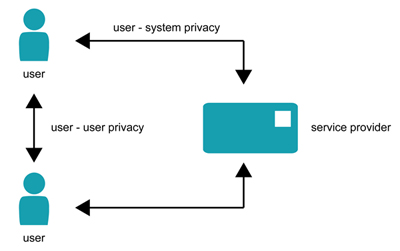
\includegraphics[scale=0.6,keepaspectratio]{fig/user-user-system-privacy}    
  \end{center}     
   \end{figure}
   
In tegenstelling tot sociale netwerken ligt bij aanbevelingssystemen het grootste probleem bij \textit{user-system privacy}. User-system privacy heeft betrekking tot de privacy kwesties tussen de gebruikers en de service provider. Een ander concept in privacy is \emph{deniability of preferences}, wat betekent dat je als gebruiker de mogelijkheid hebt om je eigen voorkeuren te ontkennen. Er is dus geen zekerheid voor een partij om de link te leggen tussen jou en je ratings.

\begin{figure}[htpb]   
    \label{Figuur::randomisatie}      
  \begin{center}    
 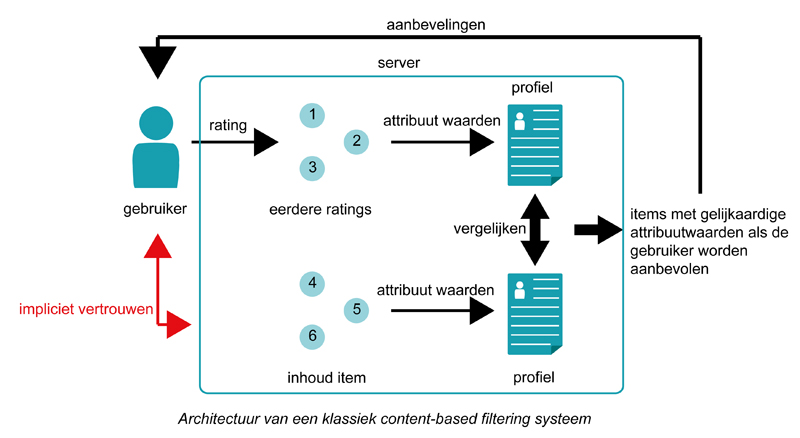
\includegraphics[scale=0.5]{fig/klassiek_systeem}    
  \end{center}   
   
   \end{figure}
Gebruikers hebben vaak een impliciet vertrouwen in de provider om verantwoord met hun data om te springen. 

\section{Betrouwbaarheid}
De betrouwbaarheid van een aanbevelingssysteem leunt dicht aan bij de privacy. Hier kunnen we de volgende vragen stellen : 

\begin{itemize}
 
\item Is het systeem voldoende beschermd tegen aanvallen van buitenaf?
\end{itemize}
 Het aanbevelingssysteem moet allereerst bestand zijn tegen aanvallen van hackers die private informatie willen bemachtigen. In het verleden is er sprake geweest van buitenstaanders die ratings manipuleerden en extra gebruikersprofielen aanmaakten om extra informatie in te winnen over het gedrag van anderen. Een voorbeeld hiervan is een vroege aanval die de correlatieco\"efficient van Pearson misbruikte. De aanval maakte gebruik van het feit dat de co\"efficient \'e\'en is als twee gebruikers identiek dezelfde ratings hebben. Er werd met behulp van een beetje informatie over de gebruiker een valse account aangemaakt waarmee de co\"efficient \'e\'en werd, zo kon men informatie halen van de ratings van de gebruiker.  Deze aanvallen kunnnen bemoeilijkt worden door een minder transparant algoritme te gebruiken dat bijvoorbeeld gebruik maakt van Singular Value Decomposition. \\Daarbuiten moet het systeem ook voorkomen dat kwaadwillige gebruikers meerdere accounts aanmaken met als doel bepaalde items te promoten of in de vergetelheid te doen belanden. 
 
 \begin{itemize}
\item Beveelt het systeem de beste items wel aan?
\end{itemize}
 
  Het kan dat een service provider enkel deze items aanbeveelt die in stock zijn of waar het systeem het meest geld op verdient en niet deze die het interessantst zijn voor de gebruiker. 
\section{Privacygevoelige data bij klassieke aanbevelingssystemen}
Veelgebruikte aanbevelingssystemen als content-based recommenders en collaborative filtering recommenders hebben toegang nodig tot persoonlijke voorkeuren om de berekeningen te kunnen doen. In de praktijk omvat dit expliciete data zoals commentaren, ratings, aankopen. Veel webapplicaties houden naast deze expliciete ook impliciete data bij zoals bezochte websites of bijvoorbeeld hoe lang een gebruiker naar een bepaald filmpje kijkt op Youtube. Ook knowledge-based recommenders verzamelen deze voorkeuren. Demografic recommenders hebben kennis nodig over de kenmerken van de gebruiker en social recommenders moeten natuurlijk weet hebben van het sociale netwerk.
\section{Privacyrisico's bij aanbevelingssystemen}
\label{sec:risicos}
\subsection{De gebruiker onderschat de omvang van de informatie die over hem wordt bijgehouden}
Van een smaakprofiel aan de hand van likes, het bijhouden van de operating systemversie met behulp van \emph{third-party} analytische tools tot het inkijken van de bezochte websites, een gebruiker is zich niet altijd bewust van de omvang van de data die van hem wordt bijgehouden\cite{pirs}. Dit is waarschijnlijk ook deels te wijten aan dat weinig gebruikers de privacyvoorwaarden lezen vooraleer een applicatie te starten. Uit een studie \cite{privdisc} bij 274 studenten bleek bijvoorbeeld 55.1\% de Facebook privacy policy niet gelezen te hebben. Hoofnagle et al. verrichte in \cite{hoofnagle} een studie over alle leeftijdsgroepen heen die hetzelfde vermoeden bevestigt. Hier blijkt  50\% van een groep van 975 personen nooit of bijna nooit de privacy policies op websites te lezen. Er is ook gewoonlijk weinig keuze, indien men de voorwaarden niet aanvaardt wordt de toegang tot de applicatie gewoonweg ontzegd. 
\subsection{Onterecht vertrouwen in de service provider}
\label{onterecht_vertrouwen}
\subsubsection{Het verkopen van data}
De informatie over de ratings en voorkeuren van gebruikers is erg interessant voor marketingdoeleinden. De verkoop van deze gegevens aan derde partijen ligt vaak niet in de lijn der verwachting van de gebruikers. Om de privacy te beschermen wordt deze data vaak geanonimiseerd. Toch biedt deze anonimisatie geen volledige bescherming. Zo hebben Narayanan en Schmatikov in \cite{Narayanan2008} de geanonimiseerde Netflix database kunnen deanonimiseren. Met een heel beperkte kennis van een gebruiker slaagden ze erin zijn records uit de databank te halen. Uit deze data konden ze politieke voorkeuren en andere gevoelige informatie afleiden.
\subsubsection{Data buiten de verwachte scope \cite{pirs}}
De gebruiker kan ervan uitgaan dat bepaalde informatie enkel zichtbaar is voor een bepaald publiek, terwijl dit niet het geval is. Er is ook geen garantie voor gebruikers dat het personeel van het aanbevelingssysteem geen kijkje neemt in hun persoonlijke data.\\

Informatie op het internet is moeilijk te verwijderen. De service provider vermoeilijkt het zelf soms aangezien er commerci\"ele waarde aan deze gegevens hangt. Het kan dus zijn dat data langer aanwezig is dan de gebruiker wil.


\section{Preventie van inbreuken op de privacy}
Nu er inzicht verkregen is welke risico's de gebruiker loopt kan er onderzocht worden wat er kan doen gebeuren inbreuken op zijn privacy te voorkomen.

\subsection{De gebruiker informeren}

Uit cijfers van Hoofnagle et al. \cite{hoofnagle} kan ook opgemaakt worden dat bij 55\% van de 975 ondervraagden de bezorgdheid rond online privacy de laatste vijf jaar is gestegen. Uit deze groep geeft 48\% aan dat de hoofdreden hiervoor is dat ze meer over de risico's ervan weten. De gebruiker informeren zou dus een positief effect kunnen hebben op zijn bezorgdheid en zijn privacy-eisen. Anderzijds gaf 77\% van de studenten in \cite{privdisc} aan dat de reden waarom de privacy policies niet gelezen werden was omdat de studenten het te veel moeite vonden of de policy moeilijk te begrijpen was. Dit toont aan dat initiatieven als "The Platform for Privacy Preferences (http://www.w3.org/P3P/)" nuttig zijn. Dit project zorgt voor een gestandaardiseerd formaat waarin websites en applicaties hun privacy policy kunnen defini\"eren. Dit formaat kan dan eenvoudig gelezen worden door een applicatie of plug-in aan de clientkant. Deze applicatie kan dan deze informatie op een gebruiksvriendelijke en begrijpbare manier tonen en eventueel op basis ervan indien de gebruiker dit wenst geautomatiseerde beslissingen nemen in zijn plaats. Zo hoeft de user de policies niet altijd te lezen. Alternatief kan de gebruiker ook bewuster gemaakt worden van de risico's die hij loopt door de privacy-informatie prominenter te tonen. Een studie van Tsai et Al. \cite{tsaitsai} toont aan dat users indien ze privacy-informatie prominent aanwezig zien meer geneigd zijn om van betrouwbaardere sites te kopen die duurder mogen zijn terwijl ze anders enkel keken naar de kleinste prijs. 

\subsection{Privacywetten}
De wetten omtrent de privacy vormt de middengrond tussen enerzijds de bescherming van de gebruiker en anderzijds de bedrijven die gerichte marketing willen voeren. Of het nu de Europese richtlijnen zijn als de Europese wetgeving rond databescherming en de Europese wetgeving rond de e-Privacy of het Amerikaanse Federal Trade Commission Act, beide lopen achter de technologie aan. Wetten worden ook vaak pas ingevoerd  nadat er iets fout is gelopen en niet om inbreuken te voorkomen.

\subsection{Privacyvriendelijke methodes}
Een alternatief is natuurlijk om met behulp van privacyvriendelijke algoritmes aanbevelingen te berekenen. Hier wordt op in gegaan de volgende hoofdstukken.

